
\newcommand{\tmstructfig}
{
\begin{fpfig}[t]{Structure of an Authorization Decision}{figure-tmstruct}
\vspace{2mm}
\begin{tabular}{cc}
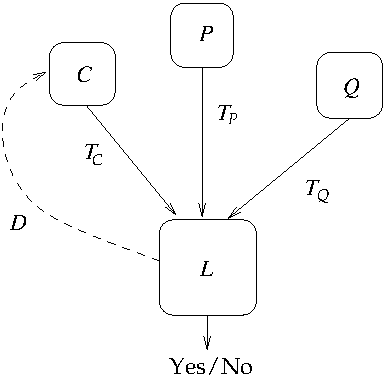
\includegraphics{tmstruct}
& 
\hspace{-10mm}
$
\begin{array}[b]{rcl}
P &:& \text{Policy}\\
C &:& \text{Certificates}\\
Q &:& \text{Authorization Query}\\
V &:& \text{Certificate Validation}\\
L &:& \text{Authorization Mechanism}\\
T_P &:& \text{Policy Compilation}\\
T_C &:& \text{Credential Encoding}\\
T_Q &:& \text{Query Compilation}\\
D &:& \text{Distributed Certificate Discovery}\\
\end{array}
$
\end{tabular}
\vspace{2mm}
\end{fpfig}
}


\newcommand{\BANrulesfig}
{
\begin{fpfig}[t]{Some Inference Rules of BAN Logic}{figure-BANrules}
\begin{mathpar}
\inferrule[message-meaning-1]
  { P \mkeyword{believes} (P \stackrel{K}{\longleftrightarrow} Q) \\
    P \mkeyword{sees} \{X\}_K }
  { P \mkeyword{believes} (Q \mkeyword{said} X) }

\inferrule[message-meaning-2]
  { P \mkeyword{believes} (\stackrel{K}{\longmapsto} Q) \\
    P \mkeyword{sees} \{X\}_{K^{-1}} }
  { P \mkeyword{believes} (Q \mkeyword{said} X) }

\inferrule[jurisdiction]
  { P \mkeyword{believes} (Q \mkeyword{controls} X) \\
    P \mkeyword{believes} (Q \mkeyword{believes} X) }
  { P \mkeyword{believes} X }

\inferrule[signature-check]
  { P \mkeyword{believes} (\stackrel{K}{\longmapsto} Q) \\
    P \mkeyword{sees} \{X\}_{K^{-1}} }
  { P \mkeyword{sees} X }
%\inferrule[nonce-verification]
%  { P \mkeyword{believes} \keyword{fresh}(X) \\
%    P \mkeyword{believes} (Q \mkeyword{said} X) }
%  { P \mkeyword{believes} (Q \mkeyword{believes} X) }
\end{mathpar}
\end{fpfig}
}


\newcommand{\ABLPinferencerulesfig}
{
\begin{fpfig}[t]{Some Inference Rules and Axioms of ABLP Logic}{figure-ABLPinferencerules}
\begin{mathpar}
\inferrule[Weaken]
{\vdash A \says (s \implies s')}
{\vdash A \says s  \implies A \says s'}

\inferrule[Speaksfor]
{\vdash A \speaksfor B}
{\vdash (A \says s)  \implies (B \says s)}

\inferrule[Ascribe]
{\vdash s}
{\vdash A \says s}

\inferrule[As]
{}
{\vdash (A \as B \speaksfor A|B) \wedge (A|B \speaksfor A \as B)}

\inferrule[Quoting]
{}
{\vdash A|B \says s \equiv A \says B \says s}
\end{mathpar}
\end{fpfig}
}


\newcommand{\AbadiSDSIaxiomsfig}
{
\begin{fpfig}[t]{Axioms of Abadi's Logic for SDSI Names}{figure-AbadiSDSIaxioms}
\begin{mathpar}
\gdesc{Reflexivity:}\,\, p \mapsto p

\gdesc{Transitivity:}\,\,
  (p \mapsto q) \implies ((q \mapsto r) \implies (p \mapsto r))

\gdesc{Left-monotonicity:}\,\,
  (p \mapsto q) \implies ((p\,\,r) \mapsto (q\,\,r))

\gdesc{Globality:}\,\,
  (p\,\,g) \mapsto g\,\, \text{if $g$ is a global identifier}

\gdesc{Associativity:}\,\, ((p\,\,q)\,\,r) \mapsto (p\,\,(q\,\,r))

\gdesc{Associativity:}\,\, (p\,\,(q\,\,r)) \mapsto ((p\,\,q)\,\,r)

\gdesc{Linking:}\,\, (p\,\,\keyword{says}\,\,(n \mapsto r)) \implies
((p\,\,n) \mapsto (p\,\,r))\,\, \text{if $n$ is a local name}

\gdesc{Speaking-for:}\,\, (p \mapsto q) \implies
((q\,\,\keyword{says}\,\,s) \implies (p\,\,\keyword{says}\,\,s))

\end{mathpar}
\end{fpfig}
}


\newcommand{\LiSDSIlogicfig}
{
\begin{fpfig}[t]{Li's Logic Program for SDSI Name Resolution}{figure-LiSDSIlogic}
\begin{center}
$$
\begin{array}{ll}
\\[-2mm]
%Linking:   & 
\mathit{contains}([A0, M0, M1|T], B) \leftarrow 
           \mathit{contains}([A0, M0], A1), \mathit{contains}([A1, M1|T], B). \\[1mm]
%Superset:  & 
\mathit{contains}([A0, M0], B) \leftarrow
               \mathit{includes}([A0, M0], SN), \mathit{contains}(SN, B). \\[1mm]
%Globality: & 
\mathit{contains}([A0, B], B) \leftarrow \mathit{isPrincipal}(B). \\[1mm]
%Self-containing & 
\mathit{contains}([B], B) \leftarrow \mathit{isPrincipal}(B). 
\end{array}
$$
\end{center}
\end{fpfig}
}


\newcommand{\PCAInferencefig}
{
\begin{fpfig}[t]{Some Inference Rules of PCA Logic}{figure-PCArules}
\begin{mathpar}
\inferrule[name\_i]
  { F }
  { \mathcal{N}(k)(F) }

\inferrule[name\_imp\_e]
  { \mathcal{N}(k)(F) \\
    \mathcal{N}(k)(F \implies G) }
  { \mathcal{N}(k)(G) }

\inferrule[signed]
  { \textrm{digital\_signature}(s, k, F) }
  { \mathcal{N}(k)(F) }

\end{mathpar}
\end{fpfig}
}


\newcommand{\TPLexamplefig}
{
\begin{fpfig}[t]{Example TPL Policy Statement}{figure-TPLexample}\tt
<GROUP NAME="Hospitals">\\
\mbox{\hspace{0.5cm}<RULE>}\\
\mbox{\hspace{1.0cm}<INCLUSION}\\
\mbox{\hspace{1.5cm}ID="reco" TYPE="Recommendation" FROM="Hospitals" REPEAT="2"/>}\\
\mbox{\hspace{1.0cm}<FUNCTION>}\\
\mbox{\hspace{1.5cm}<GT>}\\
\mbox{\hspace{2.0cm}<FIELD ID="reco" NAME="Level"/>}\\
\mbox{\hspace{2.0cm}<CONST>1</CONST>}\\
\mbox{\hspace{1.5cm}</GT>}\\
\mbox{\hspace{1.0cm}</FUNCTION>}\\
\mbox{\hspace{0.5cm}</RULE>}\\
</GROUP>
\end{fpfig}
}